\textbf{Веб-сервис 'Метод максимального правдоподобия'.}


В данной работе был разработан программный комплекс, реализующий работу с методом максимального правдоподобия. В отличии от программы из приложения А данный комплекс имеет пользовательский интерфейс, его не нужно скачивать, поскольку он является веб-ресурсом.

Рассмотрим пример взаимодействия с сервисом. На главной странице сайта пользователю предлагается загрузить в систему набор данных. Загрузить файл можно либо перетащив его в соответствующий блок, либо выбрать из всплывающего окна по соответствующей кнопке. При этом данный файл должен иметь расширение csv и быть не более 50 Мб. После валидации загруженного файла системой кнопка 'Далее' становится активной, пользователю предлагается перейти на следующий шаг. На каждом последующем шаге есть возможность вернуться на предыдущий этап с помощью навигационного меню, расположенного слева, при этом если на нем внести изменения, последующие этапы станут недоступны их будет необходимо пройти снова.

\begin{figure}[H]
    \begin{center}
        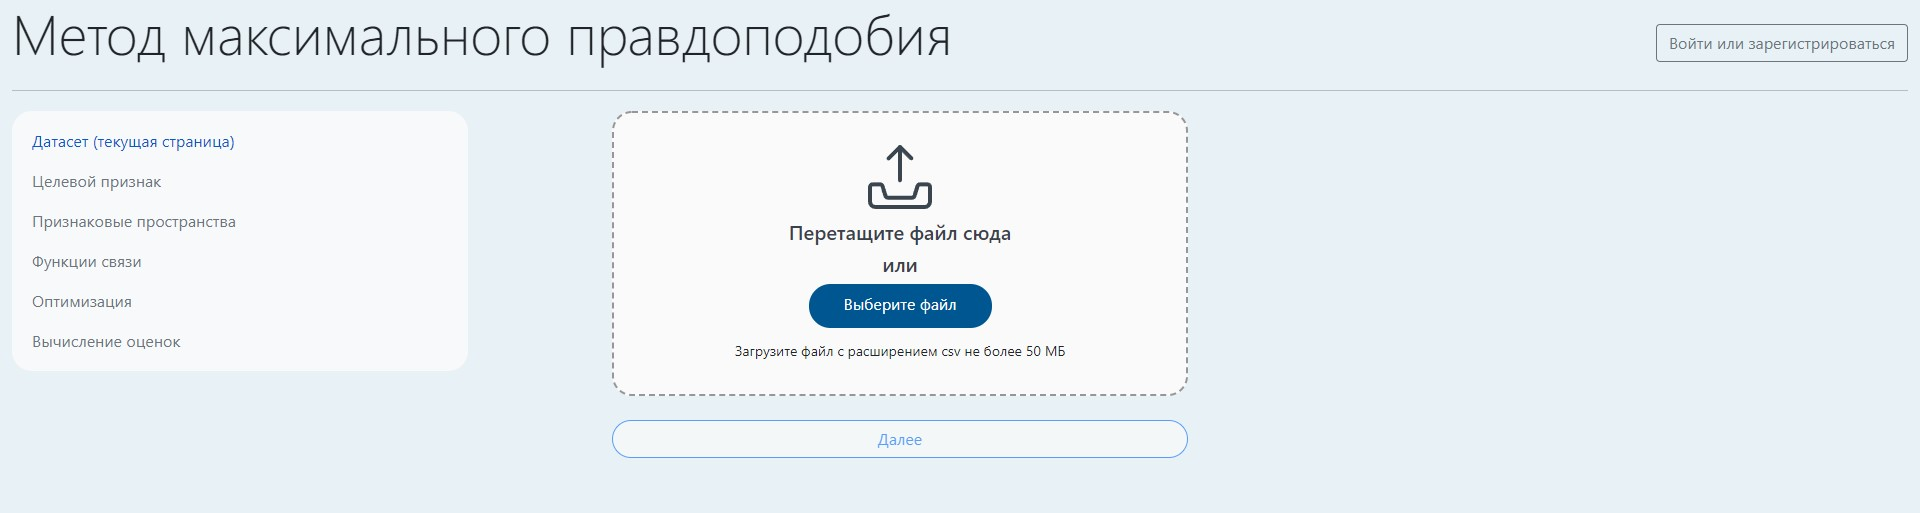
\includegraphics[width=1.0\linewidth]{src/img/screens/1.jpg}
        \caption*{Рисунок A.1 ~~ Главная страница веб-сервиса}
        \label{fig:screen_1}
    \end{center}
\end{figure}

На следующем шаге необходимо выбрать из выпадающего списка целевой признак. Признаки были получены в результате разбора загруженного пользователем файла. Также необходимо выбрать распределение целевого признака из доступных вариантов. На момент написания данной работы поддерживается 2 возможных распределения: Пуассоновское, геометрическое.

\begin{figure}[H]
    \begin{center}
        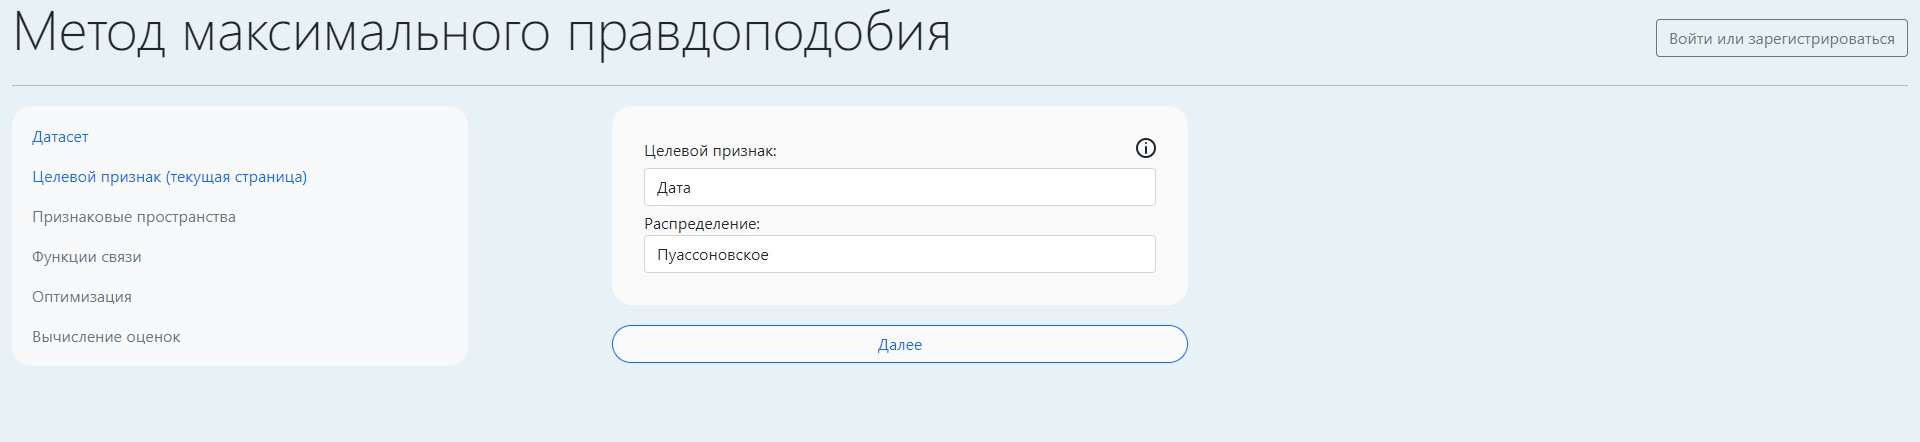
\includegraphics[width=1.0\linewidth]{src/img/screens/2.jpg}
        \caption*{Рисунок A.2 ~~ Введение целевого признака}
        \label{fig:screen_2}
    \end{center}
\end{figure}

На 3 шаге пользователю необходимо составить набор признаковых пространств. Для этого в соответствующем блоке справа выбираются необходимые признаки и вводится название данного признакового пространства. После его добавления оно отображается в центральном блоке. Для компактности в центральном блоке пишутся не названия признаков, а их порядковые номера, порядок которых определен в соответствующем списке справа.


\begin{figure}[H]
    \begin{center}
        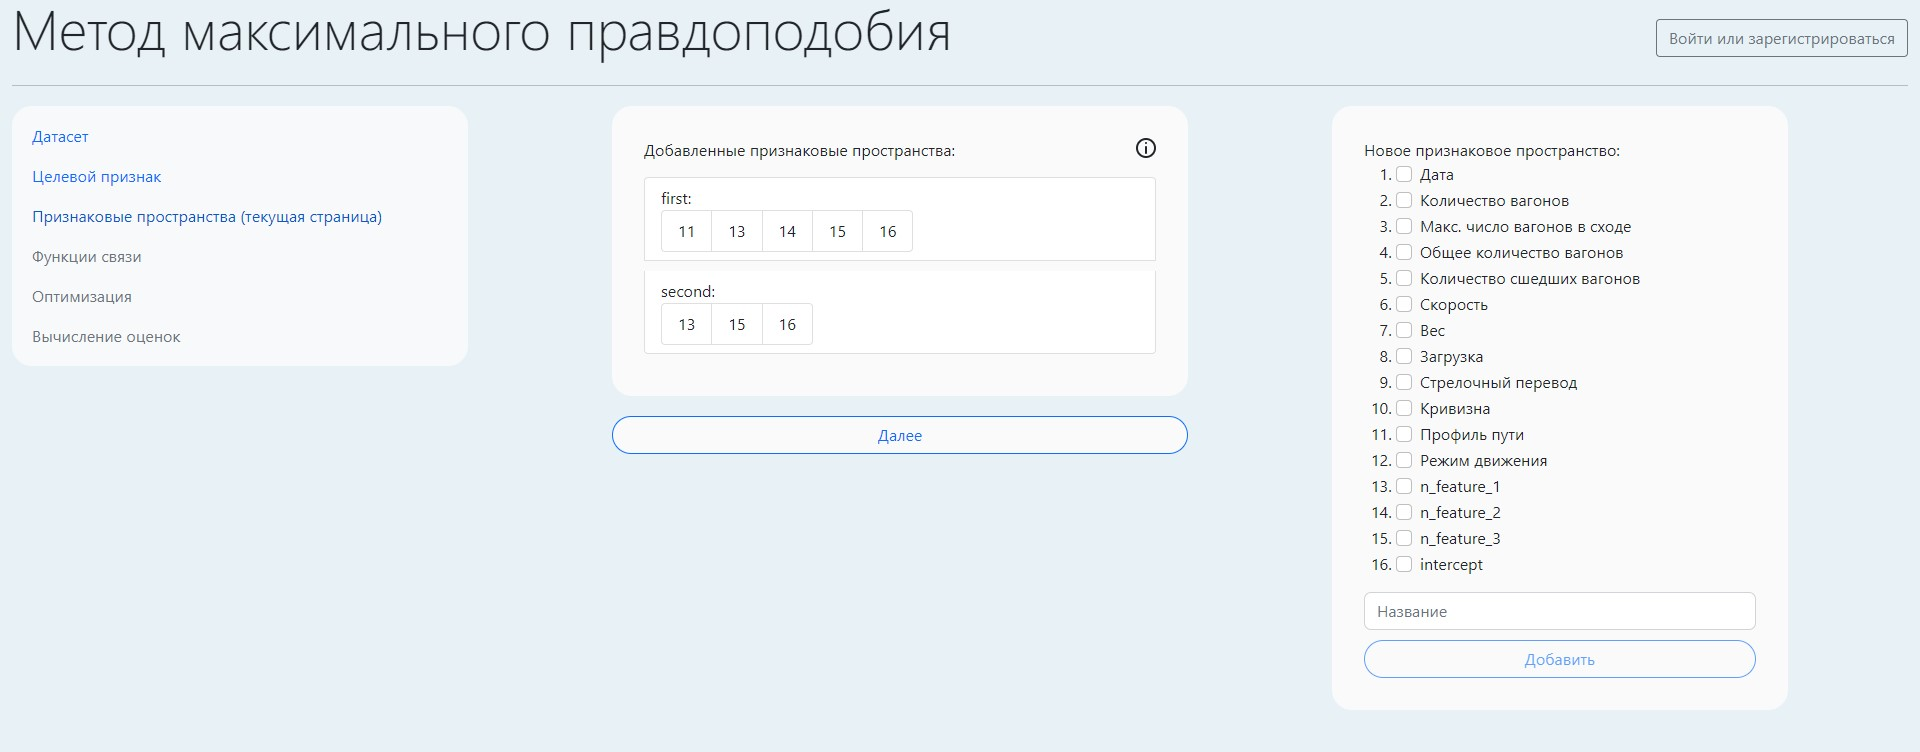
\includegraphics[width=1.0\linewidth]{src/img/screens/3.jpg}
        \caption*{Рисунок A.3 ~~ Определение признаковых пространств}
        \label{fig:screen_3}
    \end{center}
\end{figure}

После задания признаковых пространств для случаев Пуассоновской или геометрической регрессии необходимо указать функции связи. Изначально есть 2 предложенных пользователю варианта ($\exp(t), \exp(-t^2)$). В поле для ввода также есть список логарифмов функций связи, определенных в списке выше, их необходимость обусловлена техническими особенностями. Поскольку в функции логарифмического правдоподобия может присутствовать логарифм от функции связи, то предпочтительней использовать их упрощенные записи, например $-t^2$, вместо $\ln(\exp(-t^2))$. Пользователь может составить список логарифмов функций связи 'обернув' каждую функцию из списка выше логарифмом, однако для некоторых случаев метод оптимизации может не сойтись.

\begin{figure}[H]
    \begin{center}
        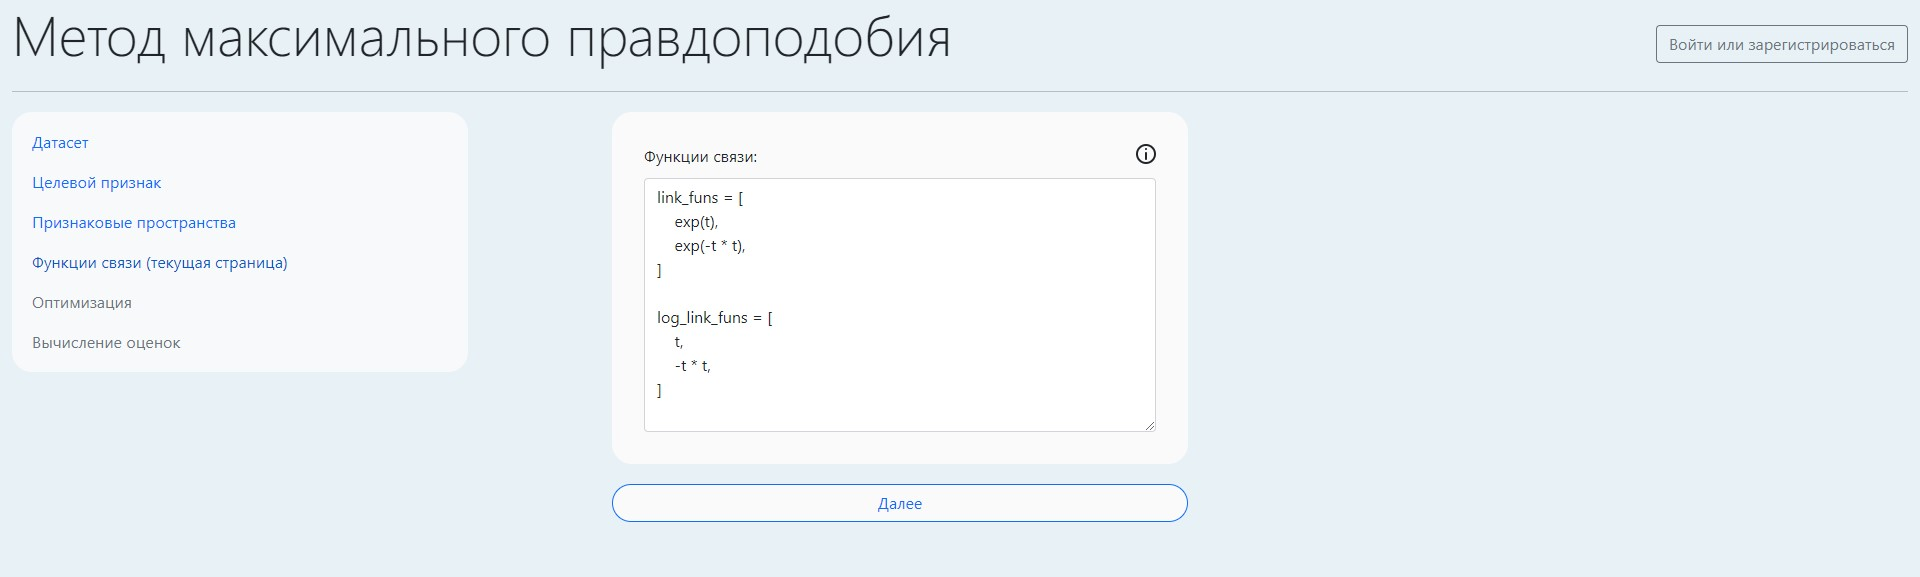
\includegraphics[width=1.0\linewidth]{src/img/screens/4.jpg}
        \caption*{Рисунок A.4 ~~ Определение функций связи}
        \label{fig:screen_4}
    \end{center}
\end{figure}

На данном этапе пользователю предлагается выбрать один из методов оптимизации из выпадающего списка.

\begin{figure}[H]
    \begin{center}
        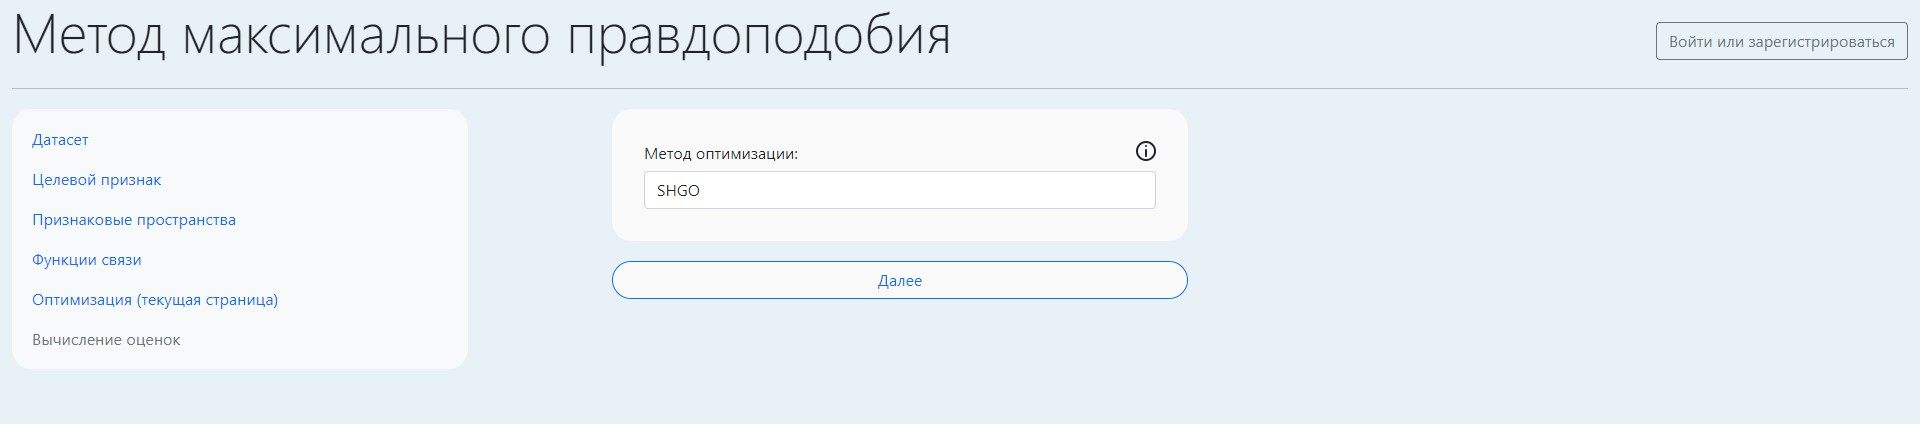
\includegraphics[width=1.0\linewidth]{src/img/screens/5.jpg}
        \caption*{Рисунок A.5 ~~ Выбор метода оптимизации}
        \label{fig:screen_5}
    \end{center}
\end{figure}

После ввода необходимых данных происходит вычисление оценок и показателей качества моделей. Пользователь может наблюдать за прогрессом вычислений по соответствующему индикатору выполнения.

\begin{figure}[H]
    \begin{center}
        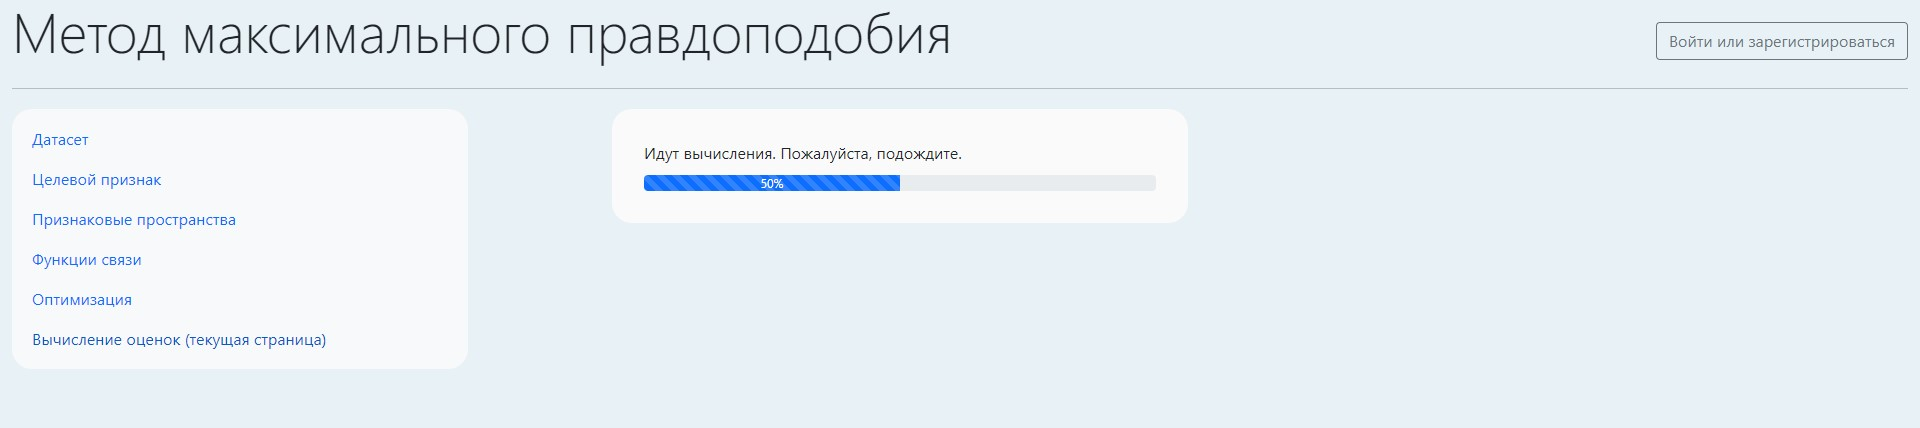
\includegraphics[width=1.0\linewidth]{src/img/screens/6.jpg}
        \caption*{Рисунок A.6 ~~ Вычисление оценок моделей}
        \label{fig:screen_6}
    \end{center}
\end{figure}

По окончании вычислений пользователю предлагается получить результаты в одном (или нескольких) форматах. На момент написания данной работы поддерживается 4 формата: json, tex, txt, pdf.

\begin{figure}[H]
    \begin{center}
        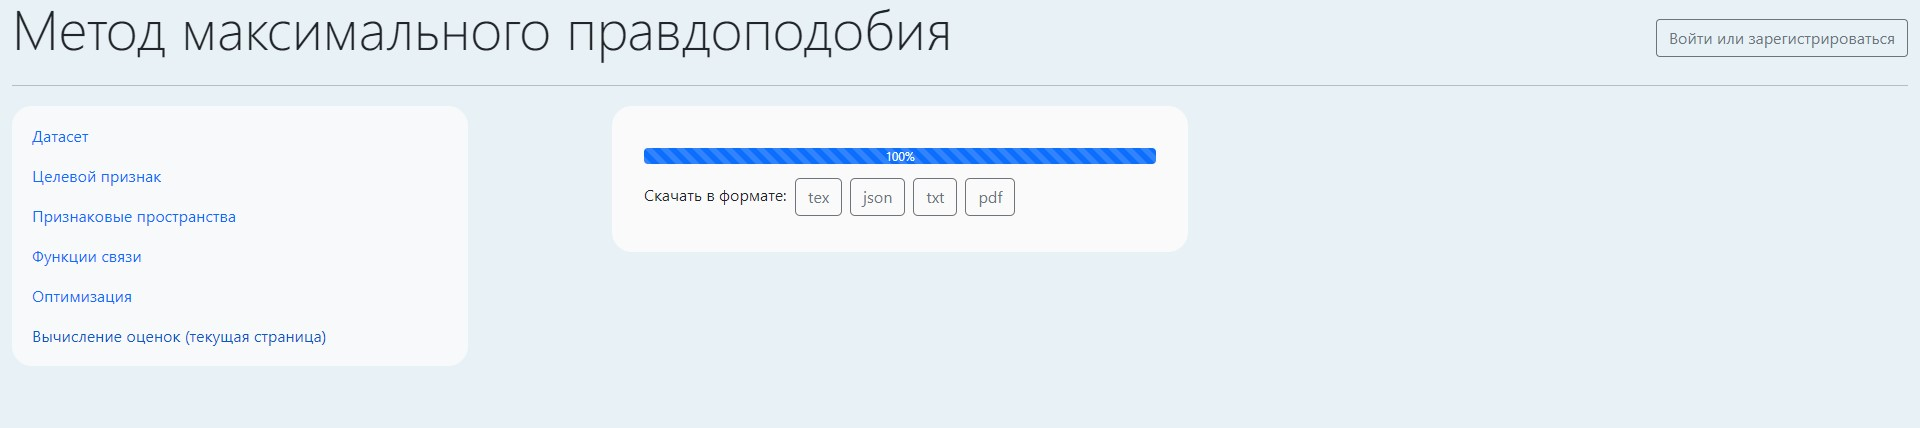
\includegraphics[width=1.0\linewidth]{src/img/screens/7.jpg}
        \caption*{Рисунок A.7 ~~ Выгрузка вычисленных оценок}
        \label{fig:screen_7}
    \end{center}
\end{figure}


\section*{Схема работы веб-сервиса}

Сервис состоит из 3-х частей. Каждая часть -- отдельный сервер. Рассмотрим все 3 части:

\begin{enumerate}[label=\arabic*.]
    \item Сервер №1 (фронтенд).
    
    Данная часть отвечает за визуальную составляющую приложения, а также за составление HTTP запросов к бекенд серверу. В качестве базового фронтенд-фреймворка был использован Angular, поэтому данный сайт реализует шаблон single-page-application, т.е. при посещении сайта пользователь загружает всего одну страницу, которая может динамически меняться. Верстка осуществлялась при помощи HTML, CSS, а также Bootstrap, благодаря которому сайт получился адаптивным под любые устройства. Макет приложения составлялся в Figma. Для написания скриптов был использован ЯП TypeScript.
    
    \item Сервер №2 (бекенд).
    
    Данная часть отвечает за внутреннюю логику приложения, скрытую от внешнего доступа и реализует архитектурный паттерн REST API.
    
    Рассмотрим пример выполнения основного запроса (вычисление параметров и оценивание моделей) к веб-сервису. После того, как пользователь ввел все необходимые данные фронтенд сервер формирует запрос к бекенд серверу. Бекенд сервер принимает данный запрос, вычисляет количество моделей, которые нужно обучить и распределяет их на группы. Для каждой группы асинхронно вызывается программа на Python, которая обучает модели и возвращает массив json объектов с информацией об обученных моделях. После завершения вычислений внутри группы на фронтенд сервер отправляется сообщение с информацией о количестве обученных моделей, после чего происходит изменение индикатора прогресса. Для двунаправленного общения между бекенд сервером и фронтенд сервером был использован протокол WebSocket.
    
    Более подробно рассмотрим устройство бекенд части:
    \begin{description}[font=$\bullet$]
        \item Java - основной язык, на котором написана серверная часть;
        \item для обучения моделей использовался язык программирования Python, программы которого вызываются из под Java;
        \item в основе приложения лежит фреймворк Spring Boot, в качестве контейнера сервлетов использовался Tomcat;
        \item для создания веб-части использовался фреймворк Spring Web;
        \item в качестве реализации протокола WebSocket был использован Spring WebSocket;
        \item для реализации системы аутентификации и авторизации, а также настройки безопасности приложения был использован Spring Security;
        \item для сбора данных о времени работы отдельных модулей, а также дополнительном логировании были использован фреймворк Spring AOP;
        \item система логирования была написана при помощи библиотеки Log4J;
        \item юнит тестирование, а также интеграционное тестирование было реализовано при помощи JUnit и Mockito;
        \item для связи с базой данных были использованы Spring Data, а также MyBatis;
        \item в качестве системы контроля версий баз данных использовался FlyWay. Таким образом при клонировании проекта не обязательно копировать базу данных, достаточно запустить DDL скрипты с FlyWay;
        \item для создания pdf файлов с информацией об обученных моделей была использована библиотека Itext7.
    \end{description}
        
    \item Сервер №3 (система управления базой данных).
    
    В качетсве СУБД использовался PostgreSQL. Базы данных были необходимы для хранения регистрационной информации о пользователях. Также пользователи, прошедшие авторизацию имеют возможность сохранять результаты своих вычислений в системе.
    
\end{enumerate}


























